% Options for packages loaded elsewhere
\PassOptionsToPackage{unicode}{hyperref}
\PassOptionsToPackage{hyphens}{url}
\PassOptionsToPackage{dvipsnames,svgnames,x11names}{xcolor}
%
\documentclass[
]{article}

\usepackage{amsmath,amssymb}
\usepackage{lmodern}
\usepackage{iftex}
\ifPDFTeX
  \usepackage[T1]{fontenc}
  \usepackage[utf8]{inputenc}
  \usepackage{textcomp} % provide euro and other symbols
\else % if luatex or xetex
  \usepackage{unicode-math}
  \defaultfontfeatures{Scale=MatchLowercase}
  \defaultfontfeatures[\rmfamily]{Ligatures=TeX,Scale=1}
\fi
% Use upquote if available, for straight quotes in verbatim environments
\IfFileExists{upquote.sty}{\usepackage{upquote}}{}
\IfFileExists{microtype.sty}{% use microtype if available
  \usepackage[]{microtype}
  \UseMicrotypeSet[protrusion]{basicmath} % disable protrusion for tt fonts
}{}
\usepackage{xcolor}
\usepackage[top=20mm,left=18mm,right=18mm,heightrounded]{geometry}
\setlength{\emergencystretch}{3em} % prevent overfull lines
\setcounter{secnumdepth}{5}
% Make \paragraph and \subparagraph free-standing
\ifx\paragraph\undefined\else
  \let\oldparagraph\paragraph
  \renewcommand{\paragraph}[1]{\oldparagraph{#1}\mbox{}}
\fi
\ifx\subparagraph\undefined\else
  \let\oldsubparagraph\subparagraph
  \renewcommand{\subparagraph}[1]{\oldsubparagraph{#1}\mbox{}}
\fi


\providecommand{\tightlist}{%
  \setlength{\itemsep}{0pt}\setlength{\parskip}{0pt}}\usepackage{longtable,booktabs,array}
\usepackage{calc} % for calculating minipage widths
% Correct order of tables after \paragraph or \subparagraph
\usepackage{etoolbox}
\makeatletter
\patchcmd\longtable{\par}{\if@noskipsec\mbox{}\fi\par}{}{}
\makeatother
% Allow footnotes in longtable head/foot
\IfFileExists{footnotehyper.sty}{\usepackage{footnotehyper}}{\usepackage{footnote}}
\makesavenoteenv{longtable}
\usepackage{graphicx}
\makeatletter
\def\maxwidth{\ifdim\Gin@nat@width>\linewidth\linewidth\else\Gin@nat@width\fi}
\def\maxheight{\ifdim\Gin@nat@height>\textheight\textheight\else\Gin@nat@height\fi}
\makeatother
% Scale images if necessary, so that they will not overflow the page
% margins by default, and it is still possible to overwrite the defaults
% using explicit options in \includegraphics[width, height, ...]{}
\setkeys{Gin}{width=\maxwidth,height=\maxheight,keepaspectratio}
% Set default figure placement to htbp
\makeatletter
\def\fps@figure{htbp}
\makeatother
\newlength{\cslhangindent}
\setlength{\cslhangindent}{1.5em}
\newlength{\csllabelwidth}
\setlength{\csllabelwidth}{3em}
\newlength{\cslentryspacingunit} % times entry-spacing
\setlength{\cslentryspacingunit}{\parskip}
\newenvironment{CSLReferences}[2] % #1 hanging-ident, #2 entry spacing
 {% don't indent paragraphs
  \setlength{\parindent}{0pt}
  % turn on hanging indent if param 1 is 1
  \ifodd #1
  \let\oldpar\par
  \def\par{\hangindent=\cslhangindent\oldpar}
  \fi
  % set entry spacing
  \setlength{\parskip}{#2\cslentryspacingunit}
 }%
 {}
\usepackage{calc}
\newcommand{\CSLBlock}[1]{#1\hfill\break}
\newcommand{\CSLLeftMargin}[1]{\parbox[t]{\csllabelwidth}{#1}}
\newcommand{\CSLRightInline}[1]{\parbox[t]{\linewidth - \csllabelwidth}{#1}\break}
\newcommand{\CSLIndent}[1]{\hspace{\cslhangindent}#1}

\usepackage{float}
\makeatletter
\makeatother
\makeatletter
\@ifpackageloaded{caption}{}{\usepackage{caption}}
\AtBeginDocument{%
\ifdefined\contentsname
  \renewcommand*\contentsname{Índice}
\else
  \newcommand\contentsname{Índice}
\fi
\ifdefined\listfigurename
  \renewcommand*\listfigurename{Lista de Figuras}
\else
  \newcommand\listfigurename{Lista de Figuras}
\fi
\ifdefined\listtablename
  \renewcommand*\listtablename{Lista de Tabelas}
\else
  \newcommand\listtablename{Lista de Tabelas}
\fi
\ifdefined\figurename
  \renewcommand*\figurename{Figura}
\else
  \newcommand\figurename{Figura}
\fi
\ifdefined\tablename
  \renewcommand*\tablename{Tabela}
\else
  \newcommand\tablename{Tabela}
\fi
}
\@ifpackageloaded{float}{}{\usepackage{float}}
\floatstyle{ruled}
\@ifundefined{c@chapter}{\newfloat{codelisting}{h}{lop}}{\newfloat{codelisting}{h}{lop}[chapter]}
\floatname{codelisting}{Listagem}
\newcommand*\listoflistings{\listof{codelisting}{Lista de Listagens}}
\makeatother
\makeatletter
\@ifpackageloaded{caption}{}{\usepackage{caption}}
\@ifpackageloaded{subcaption}{}{\usepackage{subcaption}}
\makeatother
\makeatletter
\@ifpackageloaded{tcolorbox}{}{\usepackage[many]{tcolorbox}}
\makeatother
\makeatletter
\@ifundefined{shadecolor}{\definecolor{shadecolor}{rgb}{.97, .97, .97}}
\makeatother
\makeatletter
\makeatother
\ifLuaTeX
\usepackage[bidi=basic]{babel}
\else
\usepackage[bidi=default]{babel}
\fi
\babelprovide[main,import]{portuguese}
% get rid of language-specific shorthands (see #6817):
\let\LanguageShortHands\languageshorthands
\def\languageshorthands#1{}
\ifLuaTeX
  \usepackage{selnolig}  % disable illegal ligatures
\fi
\IfFileExists{bookmark.sty}{\usepackage{bookmark}}{\usepackage{hyperref}}
\IfFileExists{xurl.sty}{\usepackage{xurl}}{} % add URL line breaks if available
\urlstyle{same} % disable monospaced font for URLs
\hypersetup{
  pdftitle={Distribuição Kumaraswamy},
  pdfauthor={Alisson Rosa,   Digite seu nome aqui!},
  pdflang={pt},
  colorlinks=true,
  linkcolor={blue},
  filecolor={Maroon},
  citecolor={Blue},
  urlcolor={Blue},
  pdfcreator={LaTeX via pandoc}}

\title{Distribuição Kumaraswamy}
\usepackage{etoolbox}
\makeatletter
\providecommand{\subtitle}[1]{% add subtitle to \maketitle
  \apptocmd{\@title}{\par {\large #1 \par}}{}{}
}
\makeatother
\subtitle{E suas Aplicações}
\author{Alisson Rosa, Digite seu nome aqui!}
\date{}

\begin{document}
\maketitle
\begin{abstract}
Muitas vezes estamos interessados em modelar variáveis que estão
definidas entre zero e um, como sabemos aonde nossa variável esta
definida mas não sabemos qual dos valores será observado, temos portanto
uma incerteza probabilística, que pode e deve ser modelada por medidas
de probabilidade. Aqui portanto, introduziremos a distribuição
Kumaraswamy, que é uma das muitas possibilidades para modelagem desse
tipo de variável, encontraremos estimativas para os parâmetros da
distribuição usando estimadores de máxima verossimilhança blah blah.
\end{abstract}
\ifdefined\Shaded\renewenvironment{Shaded}{\begin{tcolorbox}[breakable, frame hidden, borderline west={3pt}{0pt}{shadecolor}, boxrule=0pt, enhanced, interior hidden, sharp corners]}{\end{tcolorbox}}\fi

\section{\centering Introdução}

Atualmente muitos fenômenos podem ser descritos como variáveis
aleatórias (va) definidas no intervalo unitário (0,1) \footnote{Onde
  parenteses indica limites do intervalo abertos.}, assim é natural que
pesquisadores desenvolvam distribuições de probabilidade que abarcam
esse tipo de va. Uma dessas distribuições é a Kumaraswamy, que foi
introduzida em Kumaraswamy (1980) como uma alternativa ao modelo beta
para aplicações na ́area de hidrologia. Em virtude deste fato, grande
parte dos trabalhos empíricos desta distribuição concentra-se nessa área
Nadarajah (2008).

-------- DADOS EXPLICAÇÃO -------

\section{\centering A distribuição Kumaraswamy}

Vamos nessa seção introduzir quantidades básicas da distribuição
Kumaraswamy, sendo elas sua função densidade de probabilidade (pdf),
função de distribuição acumulada (cdf), função quantilica (qf), função
de verossimilhança (ll) e esperança (\textbf{E})

\subsection{Quantidade Básicas}

Seja X uma variável aleatória que segue uma distribuição Kumaraswamy,
então sua cdf é dada por:

\begin{align}
F(x;\alpha, \beta) = 1 - (1 - x^\alpha)^\beta,  \quad 0 < x< 1
\end{align}

Onde \(\alpha, \beta > 0\). Sua pdf então fica definida como:

\begin{align}
f(x;\alpha, \beta) = \dfrac{dF}{dx} =\alpha\beta x^{\alpha - 1}(1 - x^\alpha)^{\beta  - 1}, \quad 0 < x< 1
\end{align}

Sua qf, que é a função inversa da cdf, fica definida como:

\begin{align}
Q(u;\alpha, \beta) = \bigg(1 - (1 - u)^{1/\beta}\bigg)^{\dfrac{1}{\alpha}}, \quad 0<u<1
\end{align}

É FÁCIL ver que que a esperança da distribuição Kumaraswamy é dada por

\begin{align}
\text{E}(X) = \dfrac{\beta\Gamma\bigg(1 + \dfrac{1}{\alpha}\bigg)\Gamma(\beta)}{\Gamma\bigg(1 + \dfrac{1}{\alpha} + \beta\bigg)}
\end{align}

A função de verossimilhança é dada por:

\begin{align}
L(\alpha, \beta; x) = \prod_{i=1}^{n}f(x;\alpha, \beta) = \alpha^n \beta^n \prod_{i=1}^{n}x_i^{\alpha - 1}\prod_{i=1}^{n}(1-x_i^{\alpha})^{\beta-1}
\end{align}

\begin{figure}

{\centering 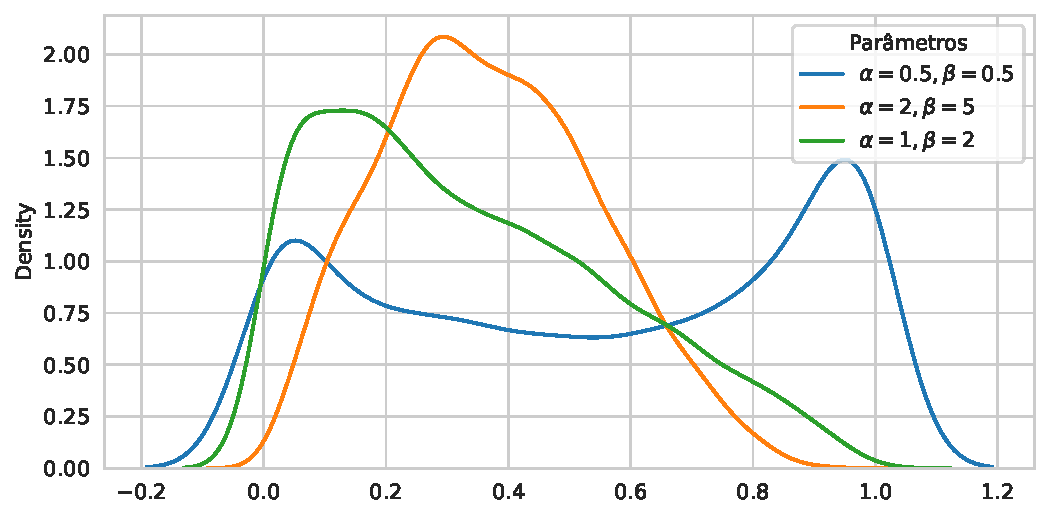
\includegraphics{report_files/figure-pdf/fig-plt-output-1.pdf}

}

\caption{\label{fig-plt}Função densidade da Kumaraswamy para alguns
valores de parâmetros}

\end{figure}

\subsection{Algumas aplicações}

\section{\centering Análise Inicial}

blah blah

\subsection{Apresentação dos dados}

\begin{figure}

{\centering 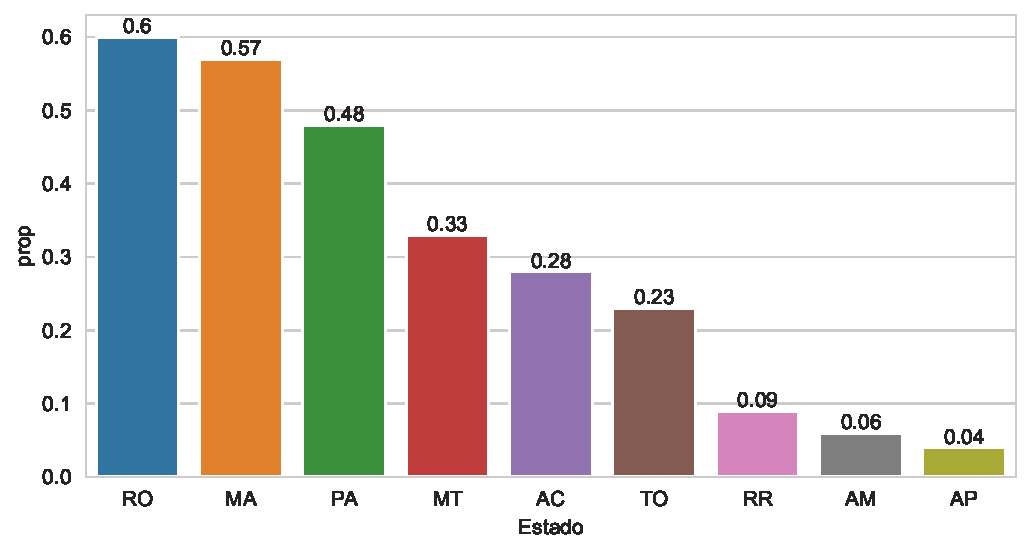
\includegraphics{report_files/figure-pdf/fig-states-output-1.pdf}

}

\caption{\label{fig-states}Proporção média dos Estados}

\end{figure}

\subsection{Medidas Básicas}

\section{\centering Ajuste do Modelo}

Explicar a relação do da verossimilhança com o ajuste do modelo

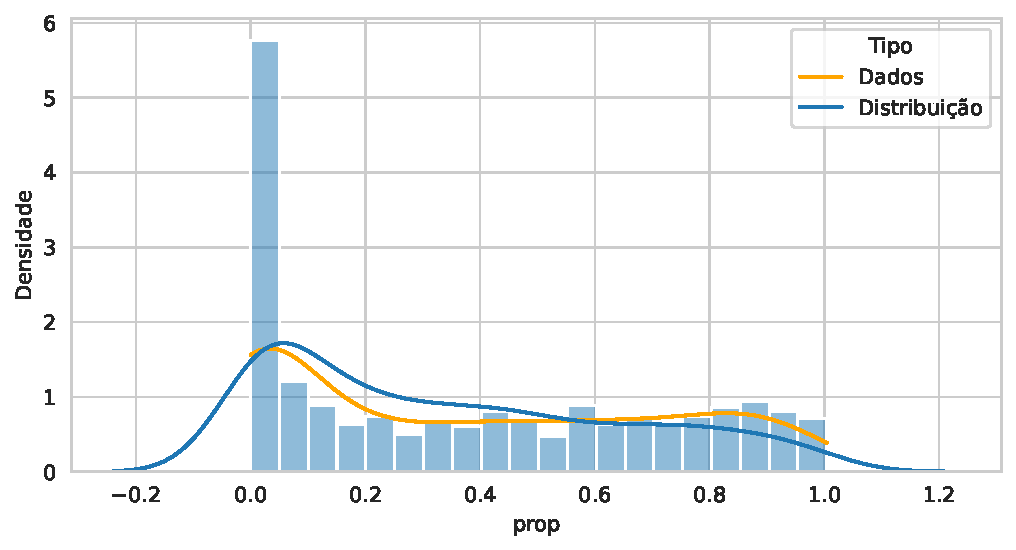
\includegraphics{report_files/figure-pdf/cell-6-output-1.pdf}

\subsection{Breve Aplicação}

\section{\centering Conclusão}

\section{\centering Referências}

\hypertarget{refs}{}
\begin{CSLReferences}{1}{0}
\leavevmode\vadjust pre{\hypertarget{ref-kuma}{}}%
Kumaraswamy, Ponnambalam. 1980. {«A generalized probability density
function for double-bounded random processes»}. \emph{Journal of
hydrology} 46 (1-2): 79--88.

\leavevmode\vadjust pre{\hypertarget{ref-nadarajah2008distribution}{}}%
Nadarajah, Saralees. 2008. {«On the distribution of Kumaraswamy»}.
\emph{Journal of Hydrology} 348 (3): 568--69.

\leavevmode\vadjust pre{\hypertarget{ref-r}{}}%
R Core Team. 2022. \emph{R: A Language and Environment for Statistical
Computing}. Vienna, Austria: R Foundation for Statistical Computing.
\url{https://www.R-project.org/}.

\end{CSLReferences}



\end{document}
